\section{Conclusion} \label{sec:conclusions}
I risultati ottenuti evidenziano come CustomNet seppur essendo una rete piuttosto semplice riesca comunque a realizzare dei buoni score. Riguardo ResNet invece i risultati sono significativamente inferiori, tuttavia bisogna tener sempre in considerazione che la rete è stata scaricata preaddestrata su immagini di tipo RGB provenienti da un altro dataset; solamente il primo e l'ultimo layer sono stati addestrati sul training set di Fahion-MNIST.\par
Entrambe le reti mostrano comunque una forte insofferenza rispetto alla classe numero 6, ovvero Shirt. Come si può vedere dalla confusion matrix questa viene confusa da CustomNet con le classi T-shirt/top, Pullover, Dress e Coat. La figura \ref{fig12:abiti_example} mostra un esempio di queste classi e si intuisce come ad esempio le classi Shirt e T-shirt/top possano risultare molto simili.
\begin{figure}[!hbt]
\centering
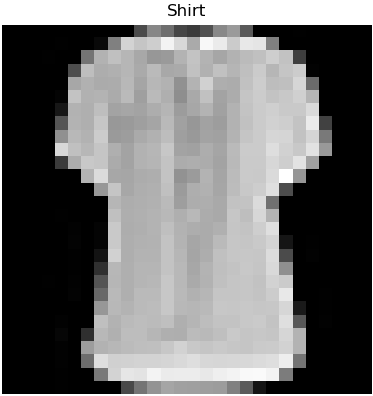
\includegraphics[width=4cm]{images/shirt6bis.png}
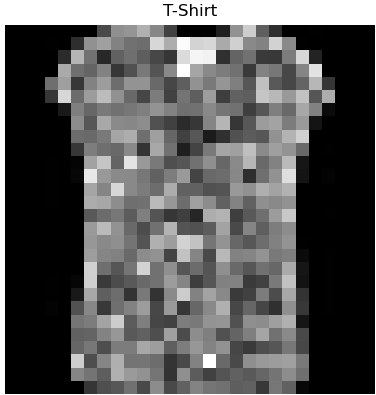
\includegraphics[width=4cm]{images/tshirt0bis.png}
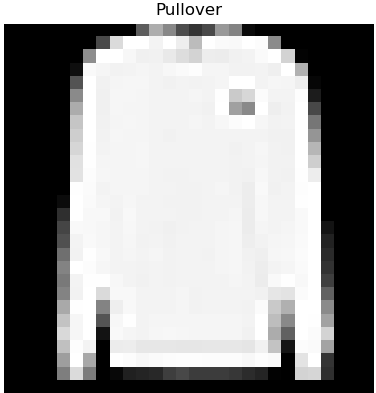
\includegraphics[width=4cm]{images/pullover2bis.png}
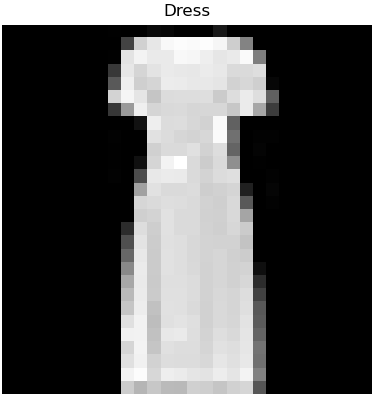
\includegraphics[width=4cm]{images/dress3bis.png}
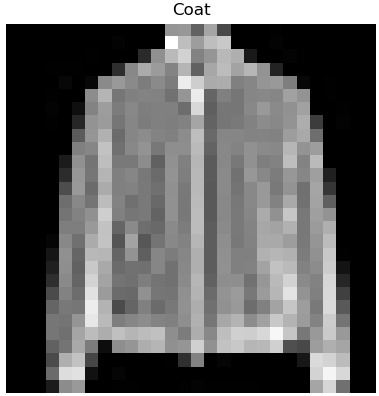
\includegraphics[width=4cm]{images/coat4bis.png}
\caption{Esempi di immagini per le classi Shirt, T-shirt/top, Pullover, Dress e Coat}
\label{fig12:abiti_example}
\end{figure}
La rete riesce invece a distinguere bene le classi riguardanti le calzature (Sandal, Sneaker, Ankle boot) seppur possano sembrare analoghe fra loro in alcuni casi.
\begin{figure}[!hbt]
\centering
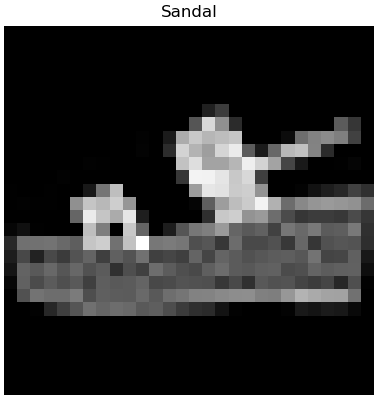
\includegraphics[width=4cm]{images/sandal5bis.png}
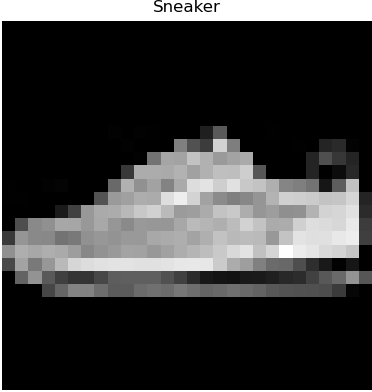
\includegraphics[width=4cm]{images/sneaker7bis.png}
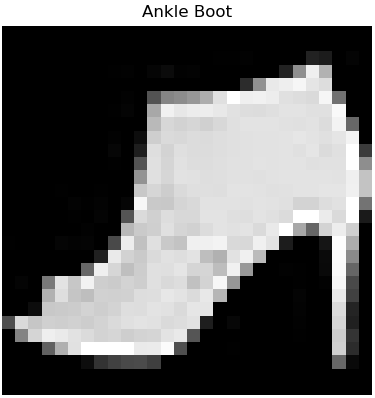
\includegraphics[width=4cm]{images/ankleboot9bis.png}
\caption{Esempi di immagini per le classi Sandal, Sneaker, Ankle boot}
\label{fig13:scarpe_example}
\end{figure}
Le immagini raffiguranti le label Trouser e Bag vengono classificate sempre in maniera corretta fondamentalmente. I due indumenti hanno infatti delle forme molto differenti rispetto alle altre classi, basta infatti osservare la Figura \ref{fig1:fashion-MNIST} a monte del documento per comprenderne le differenze.

